
\definecolor{cffffff}{RGB}{255,255,255}
\definecolor{cf2f2f2}{RGB}{242,242,242}
\definecolor{c999999}{RGB}{153,153,153}


\def \globalscale {1.000000}
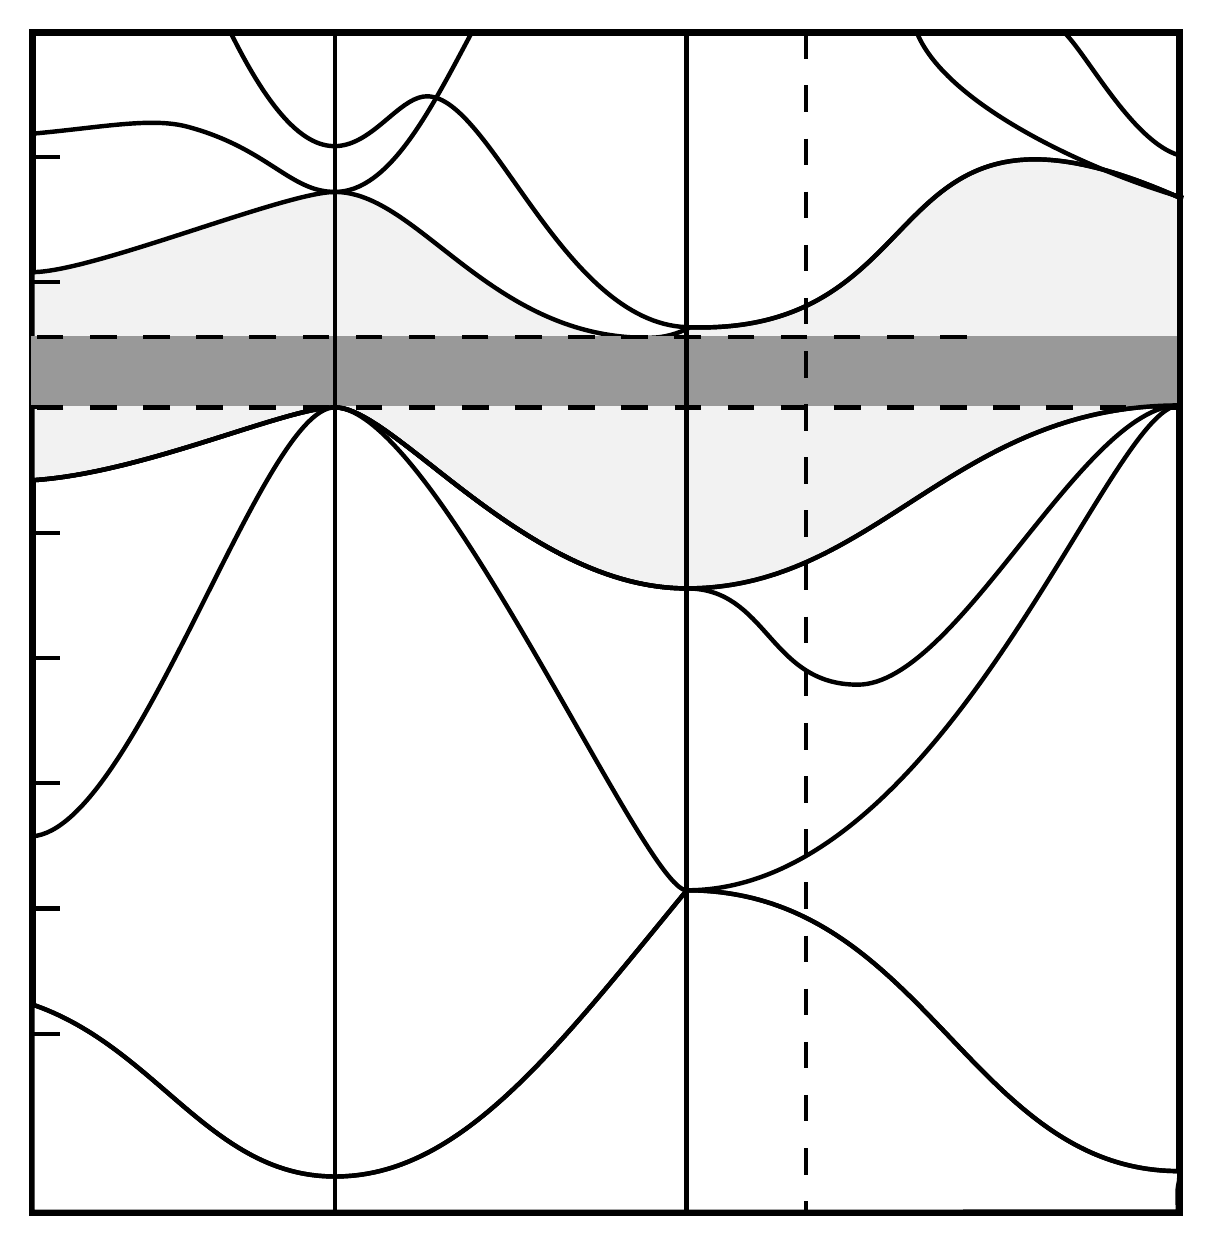
\begin{tikzpicture}[y=0.80pt, x=0.80pt, yscale=-\globalscale, xscale=\globalscale, inner sep=0pt, outer sep=0pt]
\begin{scope}% layer2
  % rect2417
  \path[draw=black,fill=cffffff,line cap=butt,miter limit=4.00,dash
    phase=5.600pt,line width=2.400pt,rounded corners=0.0000cm] (74.4173,10.0293)
    rectangle (592.4173,543.0293);


  % rect2417



  % path4525
  \path[draw=black,line join=miter,line cap=butt,miter limit=4.00,even odd
    rule,line width=1.600pt] (86.6327,66.3966) -- (73.2113,66.3966);


  % path4525



  % path3278
  \path[draw=black,fill=cf2f2f2,line join=miter,line cap=butt,miter
    limit=4.00,even odd rule,line width=1.600pt] (371.3760,143.2982) .. controls
    (365.7578,146.2680) and (359.8113,147.9695) .. (353.3475,148.0443) .. controls
    (281.3927,148.8767) and (248.8590,82.1638) .. (210.9854,82.1638) .. controls
    (188.6591,82.1638) and (101.5258,118.3832) .. (74.3892,118.3832) .. controls
    (74.3892,169.0653) and (74.3892,163.5646) .. (74.3892,212.3832) .. controls
    (124.5030,209.2610) and (188.6591,179.4549) .. (210.9854,179.4549) .. controls
    (237.8727,179.4549) and (297.8435,261.2426) .. (369.8032,261.2426) .. controls
    (455.2219,261.2426) and (489.9689,178.5844) .. (592.3893,178.5844) .. controls
    (592.3893,101.2982) and (592.4174,164.8893) .. (592.4174,84.7195) .. controls
    (453.2853,22.9971) and (488.4115,146.8284) .. (371.3760,143.2982) -- cycle;


  % path3278



  % rect4270
  \path[fill=c999999,dash pattern=on 9.60pt off 9.60pt,line join=miter,line
    cap=butt,miter limit=4.00,line width=1.600pt,rounded corners=0.0000cm]
    (73.5331,147.4532) rectangle (591.3608,178.8015);


  % rect4270



  % path4527
  \path[draw=black,line join=miter,line cap=butt,miter limit=4.00,even odd
    rule,line width=1.600pt] (86.6327,122.9680) -- (73.2113,122.9680);


  % path4527



  % path4529
  \path[draw=black,line join=miter,line cap=butt,miter limit=4.00,even odd
    rule,line width=1.600pt] (86.6327,179.3057) -- (73.2113,179.3057);


  % path4529



  % path4531
  \path[draw=black,line join=miter,line cap=butt,miter limit=4.00,even odd
    rule,line width=1.600pt] (86.6327,236.1108) -- (73.2113,236.1108);


  % path4531



  % path4533
  \path[draw=black,line join=miter,line cap=butt,miter limit=4.00,even odd
    rule,line width=1.600pt] (86.6327,292.6823) -- (73.2113,292.6823);


  % path4533



  % path4535
  \path[draw=black,line join=miter,line cap=butt,miter limit=4.00,even odd
    rule,line width=1.600pt] (86.6327,349.2537) -- (73.2113,349.2537);


  % path4535



  % path2485
  \path[draw=black,fill=cffffff,line join=miter,line cap=butt,miter
    limit=4.00,even odd rule,line width=1.600pt] (74.3892,449.2143) .. controls
    (74.3892,523.0064) and (74.3894,450.9332) .. (74.3894,542.8695) .. controls
    (193.5562,542.8695) and (426.4273,542.7672) .. (591.7851,542.7672) .. controls
    (591.0477,526.5230) and (592.4174,533.9640) .. (592.4174,524.4494) .. controls
    (497.2663,524.4494) and (477.7079,397.5994) .. (369.9005,397.5994) .. controls
    (309.4712,471.2471) and (267.3466,526.8790) .. (210.9854,526.8790) .. controls
    (154.6242,526.8790) and (130.8894,468.5689) .. (74.3892,449.2143) -- cycle;


  % path2485



  % path4537
  \path[draw=black,line join=miter,line cap=butt,miter limit=4.00,even odd
    rule,line width=1.600pt] (86.6327,405.8251) -- (73.2113,405.8251);


  % path4537



  % path4539
  \path[draw=black,line join=miter,line cap=butt,miter limit=4.00,even odd
    rule,line width=1.600pt] (86.6327,462.3966) -- (73.2113,462.3966);


  % path4539



  % path4517
  \path[draw=black,line join=miter,line cap=butt,miter limit=4.00,even odd
    rule,line width=1.600pt] (210.9854,10.0293) -- (210.9854,543.0293);


  % path4517



  % path4519
  \path[draw=black,line join=miter,line cap=butt,miter limit=4.00,even odd
    rule,line width=1.600pt] (369.8032,10.0293) -- (369.8032,543.0293);


  % path4519



  % path4521
  \path[draw=black,dash pattern=on 9.60pt off 9.60pt,line join=miter,line
    cap=butt,miter limit=4.00,even odd rule,line width=1.600pt] (423.8032,10.0293)
    -- (423.8032,543.0293);


  % path4521



  % path4523
  \path[draw=black,dash pattern=on 9.60pt off 9.60pt,line join=miter,line
    cap=butt,miter limit=4.00,even odd rule,line width=1.600pt]
    (592.3892,179.2143) -- (74.3892,179.2143);


  % path4523



  % path4568
  \path[draw=black,line join=miter,line cap=butt,miter limit=4.00,even odd
    rule,line width=1.600pt] (592.4174,524.4494) .. controls (497.2663,524.4494)
    and (477.7079,397.5994) .. (369.9005,397.5994) .. controls (309.4712,471.2471)
    and (267.3466,526.8790) .. (210.9854,526.8790) .. controls (154.6242,526.8790)
    and (130.8894,468.5689) .. (74.3892,449.2143);


  % path4568



  % path4570
  \path[draw=black,line join=miter,line cap=butt,miter limit=4.00,even odd
    rule,line width=1.600pt] (592.4174,178.5844) .. controls (560.8838,178.5844)
    and (487.6230,397.5994) .. (369.8032,397.5994) .. controls (350.9691,397.5994)
    and (255.7048,179.4943) .. (210.8432,179.4943) .. controls (177.9453,179.4943)
    and (121.0171,369.4913) .. (74.3892,373.2143);


  % path4570



  % path4572
  \path[draw=black,dash pattern=on 9.60pt off 9.60pt,line join=miter,line
    cap=butt,miter limit=4.00,even odd rule,line width=1.600pt]
    (592.3892,179.6819) -- (74.3892,179.6819);


  % path4572



  % path4574
  \path[draw=black,line join=miter,line cap=butt,miter limit=4.00,even odd
    rule,line width=1.600pt] (592.3893,178.5844) .. controls (489.9689,178.5844)
    and (455.2219,261.2426) .. (369.8032,261.2426) .. controls (297.8435,261.2426)
    and (237.8727,179.4549) .. (210.9854,179.4549) .. controls (188.6591,179.4549)
    and (124.5030,209.2610) .. (74.3892,212.3832);


  % path4574



  % path4576
  \path[draw=black,line join=miter,line cap=butt,miter limit=4.00,even odd
    rule,line width=1.600pt] (592.3893,178.5844) .. controls (548.8637,178.5844)
    and (492.2046,304.7231) .. (447.1238,304.7231) .. controls (406.9313,304.7231)
    and (406.5736,261.2426) .. (369.8032,261.2426) .. controls (297.8435,261.2426)
    and (237.8727,179.4549) .. (210.9854,179.4549) .. controls (188.6591,179.4549)
    and (124.5030,209.2610) .. (74.3892,212.3832);


  % path4576



  % path4580
  \path[draw=black,line join=miter,line cap=butt,miter limit=4.00,even odd
    rule,line width=1.600pt] (592.4174,84.7195) .. controls (452.6974,22.7363) and
    (488.6296,147.8741) .. (369.8032,143.2426) .. controls (313.9356,141.0849) and
    (281.3868,39.2221) .. (252.6732,38.9655) .. controls (231.1181,38.7691) and
    (210.9854,105.5347) .. (163.7985,10.0293);


  % path4580



  % path4582
  \path[draw=black,line join=miter,line cap=butt,miter limit=4.00,even odd
    rule,line width=1.600pt] (594.2441,84.8543) .. controls (549.6316,71.9638) and
    (485.2379,41.5859) .. (473.3738,8.9701)(273.2631,9.2679) .. controls
    (254.3226,44.7439) and (235.7612,82.1638) .. (210.9854,82.1638) .. controls
    (190.6758,82.1638) and (180.7304,62.4492) .. (144.3955,52.7133) .. controls
    (128.0894,48.3441) and (105.6619,53.0210) ..
    (74.4173,55.8515)(539.7311,9.4808) .. controls (550.1398,18.7978) and
    (571.1317,59.7002) .. (592.5151,65.6768);


  % path4582



  % path4710
  \path[draw=black,dash pattern=on 9.60pt off 9.60pt,line join=miter,line
    cap=butt,miter limit=4.00,even odd rule,line width=1.600pt]
    (496.3457,147.6819) -- (73.2916,147.6819);


  % path4710



\end{scope}
\begin{scope}% layer1
\end{scope}

\end{tikzpicture}
